\documentclass[11pt,a4paper]{scrartcl}
\setlength{\parindent}{0pt}
\setlength{\parskip}{5pt}

\newcounter{mycommentcounter}
\newcommand{\Genericcomment}[2]{%
\par%
\noindent%
\fbox{%
\begin{minipage}{0.95\textwidth}
\textsl{#1: \#\refstepcounter{mycommentcounter}%
\arabic{mycommentcounter}: #2}%
\end{minipage}%
}%
\par%
}

\newcommand{\AVTcomment}[1]{
\Genericcomment{AVT}{#1}
}

\newcommand{\SKcomment}[1]{
\Genericcomment{SK}{#1}
}

\newcommand{\HashValue}[0]{\mathsf{HashValue}}
\newcommand{\HashValVec}[0]{\mathsf{HashValVec}}
\newcommand{\CurrentWeight}[0]{\mathsf{CurrentWeight}}
\newcommand{\SuffixCode}[0]{\mathsf{SuffixCode}}

\newcommand{\Substring}[3]{#1\lbrack #2\ldots#3\rbrack}
\newcommand{\Subchar}[2]{#1\lbrack #2\rbrack}
\newcommand{\Scoretablename}[0]{\mathsf{ST}}
\newcommand{\Scoretable}[1]{\Scoretablename\lbrack #1\rbrack}
\newcommand{\Reals}{\mathbb{R}}
\newcommand{\Permname}[1]{\varphi_{#1}}
\newcommand{\Perm}[2]{\Permname{#1}(#2)}
\newcommand{\Permnameinverse}[1]{\varphi_{#1}^{-1}}
\newcommand{\Perminverse}[2]{\Permnameinverse{#1}(#2)}
\newcommand{\Alpha}[0]{\mathcal{A}}


\usepackage{amsmath}
\usepackage{amsfonts}
\usepackage{mathtools}
\usepackage{graphicx}
\usepackage{pdfpages}
\usepackage{algpseudocode}
\usepackage{algorithm}
\usepackage{palatino}
\usepackage{numprint}
\usepackage{svg}
\usepackage{comment}
\usepackage{float}
\usepackage[colorlinks=true, allcolors=blue]{hyperref}
\title{Efficient Preprocessing of Short Sequence Segments for Efficient Filtering in Comparing Protein Sequences}
\author{Anh Viet Ta (6747004)}

\begin{document}
\begin{titlepage}
\maketitle
\pagenumbering{gobble}% Remove page numbers (and reset to 1)
\thispagestyle{empty}

\textbf{Abstract:} 
\end{titlepage}
\pagenumbering{arabic}
\setcounter{page}{1}

\section{Introduction}
\section{Modern bioinformatic sequence searching and clustering}
\subsection{Recent developments}
With the advent of high-throughput sequencing technologies, the cost of genome sequencing has come down sgnificantly. Sequence databases, such as UniProt have been growing by a factor of two every two years, which leads to a significant focus on developing searching and clustering methods that can handle large-scale datasets efficiently. Algorithms and software that can scale horizontally (across multiple machines) have gained importance.

On sequence searching, new algorithms and heuristics have been developed to improve sensitivity without sacrificing speed. Tools like DIAMOND and MMseqs2 provide fast and sensitive sequence searching capabilities, especially in metagenomics and large-scale sequencing projects. HMM-based methods, such as the HMMER software, have been enhanced to improve their sensitivity and accuracy, making them invaluable for protein domain and family searching. The existing algorithms like BLAST have also seen massive improvement by using GPU parallelization and specific hardwares, namely FPGAs (Field-Programmable Gate Arrays) have been customized for accelerating sequence searching algorithms.

Recent developments on metagenomics have also given ways to specialized databases and algorithms. These databases contain sequences from environmental samples and enable the identification of novel organisms and genes within complex microbial communities.

On sequence clustering, myriads of methods have been developed. graph-based clustering methods, such as Markov Clustering (MCL) and Louvain algorithm, have gained popularity. These methods model sequences as nodes in a graph and use edge weights to represent similarities, allowing for the detection of densely connected clusters within the graph. Density-based methods like DBSCAN (Density-Based Spatial Clustering of Applications with Noise) have been applied in bioinformatics. These algorithms group sequences based on the density of data points, enabling the discovery of clusters with varying shapes and sizes. Traditional distance-based clustering algorithms, such as hierarchical clustering and k-means, have been adapted and optimized for large biological datasets. Efficient distance metrics and clustering strategies have been a focus of research.

**Deep Learning in Clustering: Deep learning techniques, particularly autoencoders and neural networks, have been explored for clustering biological sequences. These methods can learn intricate patterns and representations from raw sequence data, potentially improving clustering accuracy.

Recent Software and Tools:
**CD-HIT: CD-HIT is a widely used tool for clustering biological sequences. It allows users to cluster large datasets and select a representative sequence from each cluster based on a specified threshold.

**UCLUST: UCLUST is part of the USEARCH suite and is designed for fast sequence clustering. It uses a greedy algorithm to form clusters and is efficient for large datasets.

**MMseqs2: MMseqs2 is a software suite for sequence searching and clustering. It provides fast and sensitive sequence clustering algorithms, making it suitable for large-scale bioinformatics analyses.

**DADA2: DADA2 is a bioinformatics pipeline for the analysis of amplicon sequencing data (e.g., 16S rRNA). While it's primarily used for sequence error correction, it also involves the clustering of similar sequences into amplicon sequence variants (ASVs).

**Swarm: Swarm is a density-based clustering algorithm designed to cluster biological sequences. It's particularly useful for clustering operational taxonomic units (OTUs) in microbial ecology studies.

**HDBSCAN: HDBSCAN (Hierarchical Density-Based Spatial Clustering of Applications with Noise) is a density-based clustering algorithm that can find clusters of varying densities. It's useful for discovering clusters in datasets where clusters of different densities exist.
\subsection{MMseqs2}
MMseqs (Many-against-Many sequence searching) is a software suite for fast and deep clustering and searching of large datasets. It was published on January 6 2016 by Maria Hauser, Martin Steinegger and Johannes S\"odding. It contains three core modules: a fast and sensitive prefiltering module that eliminates most non-homologous sequences, an local alignment module based on the striped Gotoh algorithm, and a clustering module based on similary graph. Due to the modularity of the structure, it allows user to create workflows tailored to specific clustering and searching needs. The default workflow utilizes the UniProt databases to create predefined parameters and resembles the average use case. The second, cascaded clustering, clusters the input database in multiple steps, increasing the sensitivity between each steps and therefore enables finding best-hit-searches 4-10 times faster. The third workflow simply compares databases using only prefiltering and aligning modules. The last workflow updates clustering between new and old clustered database by deleting deprecated sequences and appending new sequences to each cluster.

In benchmark, MMseqs showed to be 4-30 times faster than UBLAST and RAPsearch2. MMseqs could cluster large databases down to 30\% sequence identity 2000 times the speed of BLASTclust.

%sums up the all similar \(q\)-grams (hexagrams by default) scores between query and target sequences and estimates homology by applying a z-score statistic

An improved, updated version MMseqs2 was published on June 7 2017. It boasts dramatic improvements in both efficiency and sensitivity by introducing several novel ideas. It revamped the prefiltering stage by introducing algorithm to find two consecutive, inexact \(q\)-gram matches and optimizing memory access. It also allowed the use of \(7\)-grams due to the speedup of the algorithm. %Need more

An in-depth look into the three core modules is presented below:
\subsubsection{Fast q-gram prefiltering stage}
The prefiltering stage serves to reduce the search space significantly, therefore it's imperative for the algorithm to be as efficient as possible.
Prefiltering in MMseqs2:
Input Sequences:
MMseqs2 takes a database of target sequences and a query sequence(s) as input. These sequences can be proteins, nucleotides, or any biological sequences.

Sequence Filtering:
Before prefiltering, MMseqs2 might perform basic sequence filtering, including removing low-complexity regions or sequences that are below a certain length threshold. These filtered sequences are then used in the prefiltering step.

k-mer Indexing:
MMseqs2 constructs an index of k-mers from the target sequences. K-mers are substrings of length 'k' extracted from each sequence. These k-mers serve as keys in an index data structure that allows for fast lookup. By creating this index, MMseqs2 can quickly identify potential matches for a given k-mer in the query sequence.

Query K-mer Generation:
Similarly, k-mers are generated from the query sequence. These query k-mers are used to search the index constructed from the target sequences.

Prefiltering Algorithm:
The prefiltering algorithm in MMseqs2 involves comparing the query k-mers against the indexed k-mers of the target sequences. It typically employs heuristics and cutoff values to quickly eliminate sequences that are unlikely to be significant matches. For instance, if a particular target sequence lacks a certain number of k-mers found in the query, it may be excluded from further consideration.

Score Thresholding:
MMseqs2 might employ a scoring threshold during prefiltering. Sequences that do not meet a minimum score requirement based on the prefiltering algorithm are discarded. The score is usually computed from the number and quality of matching k-mers between the query and target sequences.

Remaining Candidates:
After prefiltering, MMseqs2 retains a reduced set of candidate sequences that are likely to contain significant matches to the query sequence. These candidates undergo further, more intensive, sequence alignment steps to determine the final matches and alignments.

Output:
The final output of the prefiltering stage is a subset of target sequences that pass the prefiltering criteria. These sequences are then subjected to more detailed alignment methods to identify the most significant matches.


\subsubsection{Ungapped alignment stage}
 In MMseqs2, an additional ungapped alignment stage was introduced, where many target sequences are aligned at once using a vectorized approach. It also utilizes a linear memory access using a score matrix containing the p. Due to the extensive use of SIMD instructions, this stage achieves a linear time complexity, much more efficient compared to the Smith-Waterman alignment stage.
\subsubsection{Smith-Waterman alignment stage}
Smith-Waterman Alignment in MMseqs2:
Ungapped Alignment Results:
The Smith-Waterman alignment stage takes the output from the ungapped alignment stage as input. These are usually sequences that have shown significant similarity in the ungapped alignment but need further refinement to identify local regions of high similarity.

Local Sequence Alignment:
Smith-Waterman performs local sequence alignment by comparing all possible subsequences of the query sequence against the target sequences. Unlike global alignment algorithms (such as Needleman-Wunsch), Smith-Waterman finds the best local alignment, allowing gaps in the alignment if necessary to optimize for local similarities.

Scoring Scheme:
During Smith-Waterman alignment, a scoring scheme is employed to assign scores to matches, mismatches, and gaps. Commonly used scoring schemes include match scores for identical residues, mismatch penalties, and gap penalties for the existence and extension of gaps in the alignment.

Dynamic Programming:
Smith-Waterman algorithm uses dynamic programming to calculate alignment scores efficiently. The dynamic programming matrix is filled iteratively, and the algorithm identifies the highest scoring local alignment in the matrix.

Traceback:
Once the dynamic programming matrix is filled, the algorithm performs a traceback to identify the specific alignment path that led to the highest score. This traceback step determines the alignment positions and the alignment itself.

Alignment Score and Significance:
The alignment score obtained from the Smith-Waterman algorithm represents the quality of the local alignment. Additionally, MMseqs2 may calculate statistical measures such as E-values, indicating the expected number of alignments with similar or better scores occurring by chance in a database of a particular size.

Output:
The output of the Smith-Waterman alignment stage includes the local alignments that have passed certain score or E-value thresholds. These alignments typically contain detailed information about the matched regions, alignment scores, E-values, and possibly other statistics, depending on the specific analysis settings.

Post-Processing:
After the Smith-Waterman alignment, further post-processing steps might be applied, such as filtering out alignments below a certain score threshold, clustering similar sequences, or generating multiple sequence alignments from the obtained local alignments.

Final Results:
The final results of the MMseqs2 analysis often include the refined local alignments, which can be further analyzed or visualized based on the specific goals of the study.

It's important to note that the exact parameters, scoring schemes, and output fo
\section{Theoretical background}
Since for every alphabet \(\Alpha\), a transformer function \(f:\Alpha \rightarrow \mathcal{N}\) can be defined, mapping every character in \(\Alpha\) to a integer rank, the following sections will discuss the biological sequences not as sequences of residues, but as of transformed, coded integers.
\subsection{Optimizing target data processing}
Since the target database can be very large, a precise and efficient evaluation must be prioritized. In MMseqs2, at every residue position, relevant characters based on the user-chosen spaced seed are individually extracted from the target sequence to create a \(q\)-gram and then process these \(q\)-grams  as independent strings. This approach would incur a time complexity of \(O(q)\) to compute a hash value for each \(q\)-gram and for the complete sequence of length \(n\) this would sum up to $O((n-q+1)q)=O(nq)$.

But the \(q\)-grams are in fact not independent from each other. To create the next \(q\)-gram, one would only have to remove the first character of the previous \(q\)-gram and append the next character in the sequence. Assuming these operations are of constant time complexity, the whole process would require only $O(n+q)$ time.

This family of hashing algorithms allows efficiently enumerate hash values of all \(q\)-grams of a sequence. In order to achieve independence between hash values, the characters are usually assigned a weight, which might be expressed as $r^{q-1-i}$, where $r$, the radix, is a constant integer and $i$ is the position of the character in the $q$-gram. The calculation of a hash value from a \(q\)-gram \(w\) could then be expressed as follows:
\begin{align}
H(w) = \sum_{i=0}^{q-1}r^{q-1-i}w[i]\label{DefineHfunction}
\end{align}
where $w$ is a \(q\)-gram and $w[i]$ is the $i$-th character in $w$.
As a base case of the recursive algorithm, the hash value for the
first $q$-gram of the sequence is computed in \(O(k)\) time by evaluating
the sum defined in Equation (\ref{DefineHfunction}).
Provided we have calculated the hash value of the previous $q$-gram
\(ax\), where \(a\) is a character and \(x\) is a \((q-1)\)-gram.
Then the hash value
of the next \(q\)-gram could be computed from \(H(ax)\) and the next not yet
processed character, say \(c\). Firstly, the contribution of \(a\)
character is subtracted from the hash value. The virtual window is then
shifted right one character. This means that the weight of all characters
in \(x\) increases by a factor or \(r\). That is, we multiply by the radix.
Lastly, the new character \(c\) is added to the hash.
The hash value of \(xc\) is then calculated as follows:
\begin{align}
H(xc) = (H(ax)-r^{n-1}\cdot a)\cdot r+c\label{IncrementallyComputeH}
\end{align}
Equations (\ref{DefineHfunction}) and (\ref{IncrementallyComputeH})
provide the basic schema of recursive hashing. In implementation, the most basic form of the algorithm, called invertible integer encoding, is used, where \(r=|\mathcal{A}|\). The pseudocode for this schema is
outlined in Algorithm \ref{code:invint}.
\begin{algorithm}[t]
\caption{Invertible Integer Encoding}
\label{code:invint}
\begin{tabular}{@{}l@{~}l}
\textbf{Input:}&Encoded sequence $s$ of length $n$\\
               &alphabet size \(r=|\mathcal{A}|\)\\
\end{tabular}
\begin{algorithmic}
\State \(\HashValVec\gets []\)
\State \(\HashValue \gets 0\)
\For{\(i\) \textbf{from} 1 to $k$}\Comment{Compute 1st hash}
\State \(\HashValue \gets \HashValue \cdot r\)
\State \(\HashValue \gets \HashValue + s[i]\)
\EndFor
\State \(\HashValVec .append(\HashValue)\)
\For{\(j\) \textbf{from} 1 to $n-k$}\Comment{Compute other hash values}
\State \(\HashValue \gets \HashValue - r^{n-1}\cdot s[j]\)
\State \(\HashValue \gets \HashValue \cdot r\)
\State \(\HashValue \gets \HashValue + s[j+k]\)\
\State \(\HashValVec .append(\HashValue)\)
\EndFor
\end{algorithmic}
\end{algorithm}

In order to extend the schema to allow for spaced seeds, one could divide the seed into shorter blocks of \(q\)-grams, intertwined by blocks of "Don't Care". Each block can then be treated as individual \(q\)-gram with custom radix, and the complexity is then \(O(nb)\), where \(b\) is the number of blocks. Since the number of blocks is in worst case the weight itself, and in best case 1, recursive hashing has a same or faster time complexity than normal hashing approachs.
\subsection{Optimizing query data processing}
Given a residue alphabet \(\Alpha\) and
\(\sigma:\Alpha\times\Alpha\to\Reals\)  a score function. For
\(u,v\in\Alpha^{\ast}\), \(|u|=|v|\) is the score defined as

$$\sigma(u,v)=\sum_{i=0}^{|u|-1}\sigma(\Subchar{u}{i},\Subchar{v}{i})$$

In order to compute the $k$-environment for a \(7\)-gram efficiently, we decompose it to one group of trigram and two groups of digrams, for all of which a primary environment \(\Scoretable{u}=\lbrack (v,\sigma(u,v))\mid v\in\Alpha^{q}\rbrack\) is computed and sorted after the subscores \(\sigma(u,v))\).

The full $k$-environment of the \(7\)-gram can then be iterated as the cartesian product
\begin{align}
\Scoretable{\Substring{u}{0}{2}}\times \Scoretable{\Substring{u}{3}{4}}\times
\Scoretable{\Substring{u}{5}{6}}\label{ScoreTablesCartesian}
\end{align}
The iteration over primary environments can then stop, when it's no longer feasible to reach the threshold \(k\).

The key to improve over the method outlined in MMseqs2, is the following:

Given a bijective mapping \(\varphi:\{0,1,\ldots,q-1\}\to \{0,1,\ldots,q-1\}\). For any sequence of length \(q\),  we define a function
\begin{align}
\varphi(u)=\Subchar{u}{\varphi(0)}\Subchar{u}{\varphi(1)}\ldots\Subchar{u}{\varphi(q-1)}  
\end{align}
in that, \ \(\varphi\) permutate the residue in \(u\).

Given a special permutation \(\Permname{u}\), so that it orders the characters in \(u\): \(\Subchar{u}{\Perm{u}{i}}\leq\Subchar{u}{\Perm{u}{i+1}}\forall i, 0\leq i\leq q-2\). The resulted \(q\)-gram \(u_s\) from the permutation is then sorted \(q\)-gram and could be rearranged using the inverse function:
\begin{align}
\Perminverse{u}{\Perm{u}{i}}=i \forall i, 0\leq i\leq q-1 \Rightleftarrow \Perminverse{u}{\Perm{u}{u}}=u
\end{align}

It can be shown that
\begin{align}
\sigma(u,v)=\sigma(\Perm{u}{u},\Perm{u}{v}) \forall v\in\Alpha^{q}
\end{align}
which means, the same permutation function applied on both sequences \(u\) and \(v\)
permutates the characters in the same way and the score between the unpermutated sequences is equal to the score between the permutated. This means that the score matrix ST can be computed only for the sorted \(q\)-grams, and it would hold all scores needed to compute the full $k$-environment.

The advantage of this approach is the smaller number of sorted $q$-grams compared to unsorted, leading to a more efficient memory usage and a more compacted computation of the score matrix ST. Any overhead caused by the rearragement of the sorted $q$-grams, see Equation~\ref{Scoretableuprime}, can be reduced by SIMD instructions.
\subsubsection{Working with sorted \(q\)-grams}
\subsubsection{Enumeration}
In mathematics, a set is defined as a collection of items, where every element occurs exactly once. This definition can be expanded to multisets, where elements can occur more than once. Applying an order on these multisets, we can formalize a notion of sorted \(q\)-grams:

Given an alphabet \(\Alpha\) and a natural number \(q > 0\), a sorted \(q\)-gram over \(\Alpha\) is a multiset \(M=a_0a_1...a_{q-1}\), \(a_i\in\mathcal{A}\forall 0\leq i<q\) and \(a_i \leq a_j\forall 0\leq i < j < q\).

%The number of possible sorted \(q\)-grams for a given \(\mathcal(A)\) and \(q\) can be computed as the binomial \(\binom{q+|\mathcal{A}|-1}{q}\). The proof can be shown with induction: 
An index table of sorted \(q\)-grams can be computed recursively. Given a sorted \(q\)-gram \(u\) where the prefix of \(m\) characters is sorted and fixed, and \(u[m-1]\) has a rank of \(a_i\) then the task is to enumerate every \((q-m)\)-grams of alphabet size (\(|\mathcal{A}|-a_i\)). The induction base case is then sorted unigrams over alphabet \(\Alpha_i = \{a_j| a_j\in\Alpha \land j\geq i\}\), where there are \(|\Alpha_i|\) unigrams indexed from \(a_i\) to \(|\Alpha|-1\).

\begin{algorithm}[t]
\caption{multisetEnumerateRecursion}
\label{code:enumerateMultisetRec}
\begin{tabular}{@{}l@{~}l}
\textbf{Input:}&current multiset length \(q\)\\
               &current alphabet \(\Alpha_i\)\\
               &current prefix \(u\)\\
               &current index table IT\\
\end{tabular}
\begin{algorithmic}
\If{\(q = 0\)}
\State \(\text{IT.append}(u)\)
\Else
\For{\(a_j \in \Alpha_i\)}
\State \(multisetEnumerateRecursion(q-1,\Alpha_i \backslash [a_i,a_j),u+a_j,\text{IT})\)
\EndFor
\EndIf
\end{algorithmic}
\end{algorithm}

\begin{algorithm}[t]
\caption{multisetEnumerate}
\label{code:enumerateMultiset}
\begin{tabular}{@{}l@{~}l}
\textbf{Input:}&multiset length \(q\)\\
               &alphabet \(\Alpha\)
\end{tabular}
\begin{algorithmic}
\State \(\text{IT}\gets []\)
\For{\(a_i \in \Alpha\)}
\State \(multisetEnumerateRecursion(q-1,\Alpha \backslash [a_0,a_j),a_i,\text{IT})\)
\EndFor
\end{algorithmic}
\end{algorithm}

\subsubsection{Linear encoding}

Using the index table, a scheme to encode any given \(q\)-gram over alphabet \(\Alpha\) to its table index in \(O(q)\) can be devised. The proposition is, there exists an unique integer weight for each character \(a\) in position \(p\) so that given any sorted \(q\)-gram \(u\) over an alphabet \(\Alpha\),
\begin{align}
    c(u)=\sum_{p=0}^{q-1} w(p,u[p])\label{Equation:linearenc}
\end{align} 

encodes exactly \(u\) to its index in table IT. This can be shown with induction:

\textbf{Base case:} In case of \(q=1\), \(|\Alpha|\) unigrams can be clearly encoded with \(w(0,a) = a \forall a \in \Alpha\).

\textbf{Inductive step:} Given the above scheme is valid up until \(q\in \mathcal{N}\), it needs to be shown \(w(q,a)\) is unique for all \(a\in \Alpha\). Assuming the weight isn't unique, therefore there exist two different weights \(w_a\neq w_a'\) so that \(c(au) = w_a + c(u)\) and \(c(av) = w_a' + c(v)\) encode \((q+1)\)-grams \(au\) and \(av\) respectively, \(u,v\in \Alpha^q,a\in\Alpha\). The codes \(c(au)\) and \(c(av)\) must but differ exactly the code of their suffixes \(c(u)-c(v)\), since the \(q+1\)-grams share the same prefix. One can then formulate:
\begin{align}
    c(au) - c(av) &= (w_a + c(u)) - (w_a' + c(v))\\
    &= (w_a - w_a') + (c(u) - c(v))\\
    &= c(u) - c(v)
\end{align}
which leads to \(w_a - w_a' = 0\), or \(w_a = w_a'\), which is a contradiction.

The recursive method to then compute a \(q\times |\Alpha|\) table LE is based on the above proof. The base case can be directly given and based on index tables \(\text{IT}_{q_i,\Alpha},2 \leq q_i \leq q\), the \(q_i\)-grams are tracked for change in prefix and the weight of the prefix can be calculated with Equation~\ref{Equation:linearenc}.
\begin{algorithm}[t]
\caption{Creating linear encoding table}
\label{code:linearEncodingTable}
\begin{tabular}{@{}l@{~}l}
\textbf{Input:}&sequence length \(q\)\\
               &alphabet \(\Alpha\)\\
               &index tables \(\text{IT}_{q_i,\Alpha}\forall q_i \in [1,q]\)\\
\end{tabular}
\begin{algorithmic}
\State LE \(\gets []\)
\State LE.append(\([0,...,|\Alpha|-1]\))
\For{\(q_i\in[2,q]\)}
\State \(\CurrentWeight \gets [None \times |\Alpha|]\)
\For{\(u,i\in\text{IT}_{q_i,\Alpha}\)}\Comment{Key-Value loop}
\If{\(\CurrentWeight [u[0]] = None\)}
\State \(\SuffixCode\gets 0\)
\For{\(j \in [1,q_i]\)}
\State \(\SuffixCode += \text{LE}[j-1][u[j]]\)
\EndFor
\State \(\CurrentWeight [u[0]] \gets i - \SuffixCode\)
\EndIf
\EndFor
\State \(\text{LE}.insert(0,\CurrentWeight)\)\Comment{Place more significant weight at beginning}
\EndFor
\end{algorithmic}
\end{algorithm}

\begin{comment}
\begin{algorithm}[t]
\caption{Linear encoding of sorted \(q\)-grams}
\label{code:linearEncode}
\begin{tabular}{@{}l@{~}l}
\textbf{Input:}&sorted \(q\)-gram \(u\)\\
                &alphabet \(\Alpha\)\\
               &linear encoding table LE of size \(q\times|\Alpha|\)
\end{tabular}
\begin{algorithmic}
\State \(\text{Code} \gets 0\)
\For{\(i\in [0,q-1]\)}
\State \(\text{Code} += \text{LE}[i][u[i]]\)
\EndFor
\State return \(\text{Code}\)
\end{algorithmic}
\end{algorithm}    
\end{comment}

\subsection{Simplified approach in determining threshold}
In MMseqs, in order to evaluate a proper threshold \(k\) for the environment, a \(z\)-score statistics was applied. For each query sequence, a calibration search through a subset of 100~000 randomly sampled target sequences is performed, where the number of prefiltering operations
\begin{align}
    \text{sum}_L = \sum_{t=1}^{100~000} (L_t-k+1)
\end{align}
and its sum of scores
\begin{align}
    \text{sum}_S = \sum_{t=1}^{100~000} S_{qt}
\end{align}
are recorded. \(L_t\) here denotes the length of the target sequence \(t\) and \(S_{qt}\) the prefiltering score between query sequence \(s\) and target sequence \(t\). The expected chance prefiltering score between them is then
\begin{align}
    S_0 = (L_t-k+1)\frac{\text{sum}_S}{\text{sum}_L}
\end{align}
Assuming the number of \(q\)-gram matches is Poisson-distributed, the standard deviation of the scores \(\sigma_S\) can be computed through number of expected \(q\)-gram matches \(n_{\text{match}}\):
\begin{align}
    n_{\text{match}} &\approx \frac{S_0}{S_{\text{match}}}
\end{align}
\begin{align}
    \sigma_S &= S_{\text{match}}\sqrt{n_{\text{match}}}\\
    &= \sqrt{(L_t-k+1)\frac{\text{sum}_S}{\text{sum}_L}S_{\text{match}}}
\end{align}
where \(S_{\text{match}}\) is the expected score per chance \(q\)-gram match. The significant prefiltering score \(S_{qt}\) should then fulfill the condition
\begin{align}
    S_{qt} \geq Z_{thr}\sigma_S + S_0
\end{align}
where \(Z_{thr}\) is the significant \(z\)-score. MMseqs2 would take in a sensitivity parameter \(s\), labeled internally as the average length of \(q\)-gram list each sequence position, from the user and using a heuristic to compute for \(S_{qt}\). This approach is shown to be lacking in control for \(s\) and therefore the goal is to streamline the process and to allow for a more fine-grained control of the length of \(q\)-gram list. 

In order to approximate an appropriate threshold \(k\) for a \(q\)-gram environment, a distribution of pairwise amino acid scores is generated. This distribution is then convoluted with itself \(q-1\) times to create a distribution of unsorted-$q$-grams-vs-unsorted-$q$-grams score and the threshold can be then obtained by filtering only a fraction of the top scores. This approach could then be easily adapted for any given target amino acid distribution, where the expected probability of the \(q\)-grams is integrated into the distribution of the pairwise amino acid scores. %But since the evaluting scheme demands a score distribution between sorted and unsorted \(q\)-grams

\section{Implementation \& Design}
\subsection{Design overview}
The program consists of six main classes:
\begin{enumerate}
    \item SortedQgram, which creates a table to index every sorted q-gram of given $ScoreClass$ and $q$.
    \item MultisetEncoder, which creates a table to encode every possible sorted q-gram to integer.
    \item Distribution, which approximates a threshold $k$ for a $k$-environment given a $ScoreClass$.
    \item QgramEnvironment, which generates a score matrix between all sorted $q$-grams and unsorted $q$-grams.
    \item SpacedSeedEncoder, which generate schemes to divide spaced seed, divides them into sub-$q$-grams and encodes them into sorted $q$-gram codes.
    \item CompositeEnvironment, which is the main class. It passes sequences into SpacedSeedEncoder, uses the sorted $q$-gram codes to call individual $k$-environment and generates a Cartesian product from the environments.
\end{enumerate}
In Figure~\ref{fig:classes}, the relationship and dataflow between the classes are outlined.

\begin{figure}[t]
\begin{center}
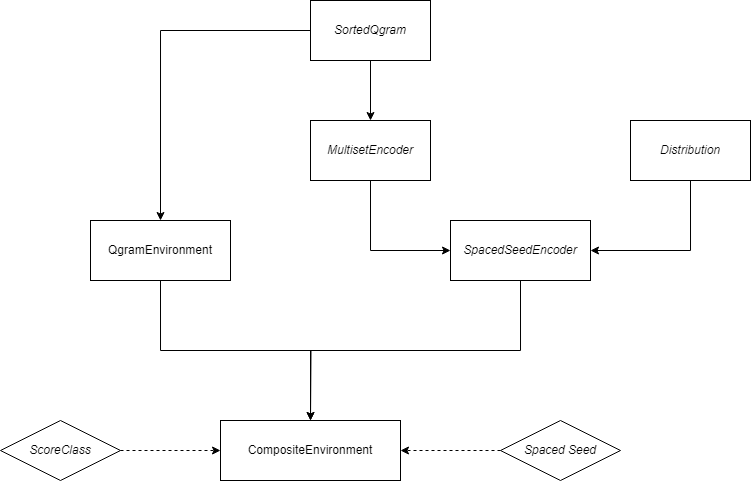
\includegraphics[scale=0.6]{graphics/Class Diagram.png}
\end{center}
\caption{Relationship between the six main classes and inputs. $Italic$ denotes compile-time evaluated classes.}
\label{fig:classes}
\end{figure}
\subsection{Input}
At compile time, the program takes in a scoring function, which in the context of protein sequences could be a BLOSUM or PAM matrix, a spaced seed and a recursive hashing function. The scoring function should detail the relevant alphabet, the transformer function, which encodes every character in the alphabet to its corresponding rank, and a matrix of scores between every pairs of characters. Internally, the spaced seed is initially represented as a numeric constant, which during computation will be transcoded into a bitset. The span of the seed can then be computed according to the position of the first 1 in the bitset and also the seed weight can be calculated by counting 1s. 

At run time the program takes in two sequence databases in FASTA format. Any data error, for example empty file or wrong data format will automatically lead to termination of the program and an error message will be logged. Additionally, the sensitivity of the program can be adjusted.

To further assist in expansion, some fixed parameters, e.g maximum sub-$q$-gram length are defined as preprocessor constants.
\subsection{Compile time computation}
Figure~\ref{fig:classes} shows that some classes/tables can be evaluated at compile time. Each seed gets transcoded and its weight and span can be precomputed and therefore, the two seed readers and their schematics can be predetermined. The two index tables for sorted/unsorted digrams/trigrams take in only scoring function as parameter and therefore, can be wholely precomputed. Since the linear encoding table LE (see Algorithm~\ref{code:linearEncodingTable}) based solely on the sorted digrams/trigrams index table, it also can be evaluated at compilation.
\subsection{Run time computation}
Internally the spaced seed is stored and represented as a 64-bit constant integer. The first step to process this spaced seed is a conversion to a bitset. Its span could then be determined as the length of the bitset subtracted by the position of the most significant 1-bit and its weight is then obtained by iterating over its span.

The program also creates a scheme to divide the spaced seed. The position of the heavier primary environments (if any) is placed at the earlier portion of the spaced seed.

In order to prepare for the recursive hashing of the target sequences, the spaced seeds are also divided in $b$ blocks of smaller $q$-grams. The complexity of the recursive hashing of a sequence of length $n$ is $O(nb)$.
In the implementation of MMseqs2, a mechanism to evaluate the surrounding of current position while iterating the query sequences is introduced. The idea of this mechanism is to adjust the threshold of the \(q\)-gram environment in response to regions where local composition varies considerably from the background distribution. Without adjusting, these low regions can lead to biases in the prefiltering result. This correction of the threshold can be summarized as follow:
\begin{align}
    \Delta S_i(u[i]) = \sum_{a=1}^{|\mathcal{A}|}f(a)\sigma(a,u[i])-\frac{1}{2d}\sum_{j=i-d,j\neq i}^{i+d}\sigma (u[i],u[j])
\end{align}
where \(u\) is the query sequence, \(i\) the current residue on the sequence and \(f(a)\) the background frequency of residue \(a\).

The minuend is a representation of the expected score resulting from the background distribution, which can be precomputed when the target data is read. The subtrahend involves the current region in the query sequence and introduces a parameter \(d\) for the radius of the region, defined in MMseqs2 as a constant 20.

The corrected score can then be computed as the sum of the pairwise amino acid score and the score correction. In the implementation, this correction is subtracted from the threshold at the beginning of the computation.

An issue in enumerating the Cartesian product is the possible difference in number of loops (e.g 2 loops for seed weight 4-6, 3 loops for seed weight 7). To resolve this problem and allow the easy expansion to greater seed size, a flexible loop structure is designed, where an array containing the loop indexes is created. The earliest entry of the array holds the most outer loop index and the later an entry is, the more inner the loop index the entry holds. By iterating through only the most outer loop and only adjusting the inner loop indexes as needed, the scheme can account for any number of loops.

The formulation of the loop structure, along with the integration of background score correction, is outlined in the pseudocode below:

\begin{comment}
\begin{algorithm}[t]
\caption{Merging query and target data}
\label{code:merging_data}
\begin{tabular}{@{}l@{~}l}
\textbf{Input:}&query data \(query\)\\
               &target data \(target\)
\end{tabular}
\begin{algorithmic}
\For{\(i\) \textbf{from} 1 to $|\mathcal{A}|$} \Comment{Generate random
integers for each character}
\State \(f(A[i]) \gets \mathsf{RandomInteger}()\)
\EndFor
\For{\(i\) \textbf{from} 1 to $|\mathcal{A}|$} \Comment{Generate lookup
table to remove character}
\State \(f_r(A[i]) \gets \rol(f(A[i]),k-1)\)
\EndFor
\State \(\HashValue \gets 0\)
\For{\(i\) \textbf{from} 1 to $k$} \Comment{Compute first hash value}
\State \(\HashValue = \rol(\HashValue,1)\)
\State \(\HashValue = \XOR(\HashValue,f(s[i]))\)
\EndFor
\State \(\mathsf{process}(\HashValue)\)
\For{\(j\) \textbf{from} 1 to $n-k$} \Comment{Compute other hash values}
\State \(\HashValue = \XOR(\HashValue,\rol(f(s[j]),k-1))\)
\State \(\HashValue = \rol(\HashValue,1)\)
\State \(\HashValue = \XOR(\HashValue,f(s[j+k])\)
\State \(\mathsf{process}(\HashValue)\)
\EndFor
\end{algorithmic}
\end{algorithm}
\end{comment}

\subsection{Merging target and query data}
After being collected, the hashed data from the target and query sequences are packaged as byte units, prioritizing hash values. They then get sorted individually using radix sort (see GTTL), resulting in two data vectors sorted by hash values which would then be merged value by value, skipping through unmatching blocks.

\begin{algorithm}[t]
\caption{Merging query and target data}
\label{code:merging_data}
\begin{tabular}{@{}l@{~}l}
\textbf{Input:}&query data \(query\)\\
               &target data \(target\)
\end{tabular}
\begin{algorithmic}
\State \(target\_idx \gets target.start\)
\State \(query\_idx \gets target.start\)
\While{\(target\_idx \neq target.end\) \(\land\) \(query\_idx \neq query.end\)}
\State \(target\_hashval \gets target[target\_idx].hashval\)
\State \(query\_hashval \gets query[query\_idx].hashval\)
\If{\(target\_hashval < query\_hashval\)} \Comment{Skipping on target vector}
\While{\(target[target\_idx].hashval = target\_hashval\)} 
\State \(target\_idx++\)
\EndWhile
\Else
\If{\(target\_hashval > query\_hashval\)} \Comment{Skipping on query vector}
\While{\(query[query\_idx].hashval\)} 
\State \(query\_idx++\)
\EndWhile
\Else \Comment{Match found}
\State \(target\_block\_end = target\_idx\) 
\While{\(target[target\_block\_end] = target\_hashval\)}
\State \(target\_block\_end++\)
\EndWhile
\State \(query\_block\_end = query\_idx\)
\While{\(query[query\_block\_end] = query\_hashval\)}
\State \(query\_block\_end++\)
\EndWhile
\State \(create\_matches([target\_idx,target\_block\_end),[query\_idx,query\_block\_end))\)
\EndIf
\EndIf
\EndWhile
\end{algorithmic}
\end{algorithm}

The merging process results in a vector of matches, represented again as byte units, containing respectively the sequence number of the match on the target, on the query, the diagonal number (difference between the target and query sequence position), and the query sequence position. These quartets are again sorted with radix sort to prepare for ungapped alignment stage.
\section{Benchmark \& Performance}
\subsection{Determining threshold}
\subsection{Performance}
\subsubsection{Overall execute time performance}
\subsubsection{Execute time performance analysis}
\subsubsection{Dependence of execute time on acceptance rate}
\subsection{Possibility of expanding seed}
\section{Discussion \& Future improvements}
\subsection{Scalability}
\subsection{Full compile-time calculation of environments}
\section{Conclusion}
\section{Reference}

\end{document}
